\documentclass[11pt]{article}
\usepackage[T1]{fontenc}
%^\usepackage[utf8]{inputenc}
\usepackage{amsmath,mathrsfs,bm}
\usepackage{color}
%\usepackage{cleveref}
\usepackage{mathtools}
\usepackage{graphicx}
\usepackage[font=footnotesize,labelfont=bf]{caption}

\usepackage{natbib}
\usepackage[superscript,biblabel]{cite}

%\usepackage{fullpage}
\usepackage[margin=0.5in]{geometry}

\pagenumbering{gobble}

\usepackage{fontspec}
\setmainfont{Arial}

% \linespread{1.05}
\newcommand{\jb}[1]{{\color{blue} (#1)} }
\newcommand{\gs}[1]{{\color{red} #1}}
\begin{document}




\subsection*{Significance and Background}

A large proportion of common diseases (i.e. prevalence > \jb{XX}\%) are genetically complex. In contrast to Mendelian diseases, genetic causation of complex diseases is not straightforward, with genetic risk for any given disease spread across a large number of genes, each individually of relatively minor effect. While successful efforts to map the genetics of Mendelian diseases date well back into the $20^{th}$ century, only in the past decade with the maturation of the genome wide association study (GWAS) approach has some understanding of the genetic basis of complex disease begun to emerge\cite{Visscher:2012je,get_more}. It's become clear now that estimates of heritability based on the twin study design were broadly accurate (if slightly overestimated in some cases), and that the heritabilities of common complex diseases are generally high. GWAS and related approaches have also shown that a substantial proportion of the variance in risk can be attributed to a very large number of common alleles \cite{Consortium:2009ef, Lee:2012iu,Loh:2015hz, Ripke:2014eb}, while sequencing and exome studies indicate a role for rare variants of large effect as well \cite{Richards:2016cs, Genovese:2016fv, Purcell:2014gw}. The totality of the evidence therefore suggests that thousands or perhaps even tens of thousands of individual genetic variants play a role in determining susceptibility to any given complex disease. Less clear however is our understanding of the forces which govern the prevalence and genetic architecture (i.e. the relationship between allele frequency and effect size) of complex disease. In contrast to Mendelian diseases, where nearly a century of theory explain how mutation rate, dominance, selection \cite{Patil:2010ha} and demography \cite{HurlesText} combine to influence the prevalence of these diseases, there is relatively little in the way of quantitative theory on the evolution of complex disease. 

% \jb{need to introduce idea of variation in prevalence and architecture as tool to greater understanding}
% Variation in the prevalence of diseases with similar fitness costs may then simply be down to difference in their mutational target sizes, and variation in genetic architectures may arise chiefly from differences in the distribution of mutational effect sizes. Conversely, variation in the fitness costs of specific diseases will lead to differences in the strength of direct selection against risk incresing variants associated with those diseases, which should account for some amount of variation in both architecture and prevalence.


Nonetheless, several qualitative mechanisms have been proposed which may potentially explain the observed patterns. Perhaps the most straightforward is that the present distribution of genetic risk reflects a simple balance between mutation and selection \cite{Johnson:2005do}. The prevalence of common disease may therefore be ascribed to relatively large mutational target sizes for many diseases. Variation among diseases in their prevalence and genetic architectures may simply reflect difference in features such as the mutational target size, distribution of effects, and fitness cost of the disease. The direct selection experienced by a given allele is likely only part of the story, however, as the extreme polygenicity of complex diseases indicate that pleiotropy must almost surely be extensive \cite{Pickrell:2016ko, Visscher:2016fp}. Indirect selection due to these pleiotropic effects may therefore play a major role in determining architecture and prevalence, both in steady-state scenarios, where pleiotropic effects may alter the stregth of selection for or against disease alleles or under more dynamic hypotheses, where recent positive selection on a trait genetically correlated to disease may have altered prevalence and/or architecture, as has been argued in a number of cases with conflicting evidence \cite{Fraser:2013jj,Berg:2014bs, Corona:2013cl, Chen:2012jv, Ayub:2014hk,Polimanti:2017bv}. Alternative explanations invoke the recent and profound changes in the human environment (diet, lifestyle, etc.) and the possibility that the mismatch between the ancestral human environment and present conditions that have resulted in a large increase in disease prevalence \cite{Gibson:2000vi, Gibson:2009ie}. Such was the original basis for the ``thrifty genotype'' hypothesis \cite{Neel:1962tj, Neel:1999tu}, and subsequent observation of large scale oscilations in type 2 diabetes incidence in response to food shortage and economic crisis and subsequent recovery in Cuba in the 1990s \cite{Franco:2013hb} indicate that this effect can be profound indeed. While some of these ideas likely apply to some diseases (and they are also not mutually exclusive), more often than not they have been put forward as verbal models only, and so it is difficult to quantitatively check their predictions.

Each of these hypotheses are ultimately statements about population and quantitative genetic processes. While some models relating population genetic processes with the kind of data emerging from GWAS have been proposed, they generally rely on various \textit{ad hoc} or limiting assumptions that make easily interpretable inference difficult. Nonetheless, two studies in particular have been especially influential. Pritchard, in 2001\cite{Pritchard:2001hw}, considered a model in which the effect on disease risk is completely uncoupled from their fitness cost, i.e. an extreme pleiotropy limit. While this paper was enormously influential in grounding the debate surrounding the common disease-common variant hypothesis in population genetic theory\cite{Pritchard:2002ux}, it seems unrealistic that a mutation's effect on disease risk should not have any consequences for its fitness. A second study which has been influential is that of Eyre-Walker in 2010 \cite{EyreWalker:2010dn}, who posited that all mutations are deleterious \textit{a priori}, but arbitrarily assumed a relationship between effect size and selection coefficient of the form $\alpha =\delta S^\tau (1+\epsilon)$, where $S$ is the selection coefficient, $\delta$ is a randomly chosen sign (i.e. $1$ or $-1$), $\epsilon$ is a noise term, and $\tau$ is a ``coupling parameter'' meant to capture the effect of pleiotropy: where $\tau =1$ means no pleiotropy and $\tau=0$ gives Pritchard's \cite{Pritchard:2001hw} extreme pleiotropy limit. While this model has seen empirical application (see Specific Aim 2 below for more background on the Eyre-Walker model in this context), it does not have any obvious theoretical justification, and indeed possesses some odd features, such as fitenss equivalence of mutations with opposing effects on disease. While these studies have both been extremely influential, it seems worth reemphasizing the fact that neither posesses any concept of fitness surface relating an explicit disease phenotype to natural selection, and in light of our rapidly accumulating knowledge of the genetic architecture of complex disease, a fresh take on the problem seems due. 

Here I propose to develope generative models for the way that genetic architecture and disease prevalence will be affected by evolutionary parameters such as mutation, natural selection, pleiotropy and demography. I will develop these models into statistical inference approaches which take advantage of the rich information present in GWAS data to infer the underlying parameters which govern the evolution of complex disease genetic architecture.

% Given the influence these studies have had, the value in genetic models of complex disease which are grounded in population genetic and evolutionary quantitative genetic principles seems clear, and that is the focus of the presently proposed research. I will develop and analyze explicit population genetic models of complex disease evolution, exploring the roles of variation in mutational target size, environmental change, pleiotropy, and non-equilibrium demography in shaping the distribution of complex disease risk within human populations. This modeling work will be leveraged into a framework to infer the factors which are responsible for variation in the genetic architecture of complex diseases from GWAS data for a range of diseases.

\subsection*{Approach}
\paragraph{Preliminary Results}
Our simplest model and point of departure considers the impact of mutation and selection on a single disease in a constant environment. In this model, each individual's risk of developing disease is a non-linear transform of an underlying (and generally unobserved) disease liability trait, such that
\begin{align}
  R=\ell(Z),    \qquad    Z = \sum_{i}\alpha_ig_i + \epsilon
\end{align}
where an individual's liability for disease ($Z$) is an additive trait, $\alpha_i$ and $g_i$ are liability scale effect size and genotype respectively at site $i$, and $\epsilon$ is a normally distributed deviate which captures stochastic variation in risk among genotypes with the same mean liability, (i.e. the ``environment'' of classical quantitative genetics). An individual's probability of developing disease (i.e. their ``risk'': $R$) is a monotonic function of their liability. This form covers a range of standard models for the genetics of binary traits, including Wright's liabity threshold model\cite{Wright:1934wd,Lush:1948vc,FalconerAndMcKay,Falconer:1965bn}, the logistic model commonly employed in GWAS\cite{Risch:1996ub}, and the exponential of Risch's multiplicative model \cite{Risch:1990ty}, among other possibilities (the difference among these is simply in the choice of the monotonic function $\ell$). Previous work \cite{Slatkin:2008hw, Wray:2010ir} suggests that the exact choice of $\ell$ is unlikely to be particularly important, and our preliminary investigations (omitted due to space constraints) support this conclusion. As such I will take $\ell$ to be the probit link function of Wright's liability threshold model for the remainder of this proposal, though I will explore other choices to understand what impact if any they might have on our results.

The number, frequencies and effect sizes of the sites contributing to variation in liability arise from population genetics processes. Liability increasing and decreasing mutations arise according to an infinite sites model with free recombination among sites at genome wide rates $\mu^+$ and $\mu^-$, with effect size distributions $f^+\left(\alpha\right)$ and $f^-\left(\alpha\right)$ respectively. Individuals with the disease have a reduced fitness of $1-S$ (disease free individuals have fitness 1).

The genetic architecture of the disease under this simple model is shaped by mutation-selection-drift balance, and can be related to standard results from quantitative genetics. The steady state is reached when
\begin{align}
  U^+ = U^- + V_A \underbrace{S\phi\left(\Phi^{-1}\left(1-P\right)\right)}_{\text{selection gradient}}
  \label{univariate-bulk-eq}
\end{align}
where $U^+ = \mu^+\int_{0}^{\infty}\alpha f^+\left(\alpha\right)\mathrm{d}\alpha$ is the total per generation mutational increase in liabilty (with $U^-$ defined similarly as mutational pressure toward decreased liability). The final term accounts for the selection pressure toward lower liability; $V_A$ is the additive genetic variance of liability, $P$ is the disease prevalence, and $\phi$ and $\Phi$ are the Gaussian pdf and cdf repsectively. The compound term multiplying $V_A$ is a selection gradient in the standard quantitative genetics sense, and is a simple generalization of the gradient exerted by truncation selection to cases where the ``truncated'' individuals have fitness greater than zero  \cite{Charlesworth}.

The steady state requirement allows us to derive expressions for any summary of genetic architecture. While the mutation rates, effect size distributions, and fitness cost of the disease are biological inputs, disease prevalence ($P$) and genetic variance ($V_A$) are dependent variables which evolve as part of the system. The additive genetic variance, as a product of the genetic architecture, depends on how the frequencies of individual alleles evolve, which depends on the individual selection coefficients they experience. An individual allele with effect size $\alpha$ on disease liability will experience a selection coefficient
\begin{align}
  s = -2\alpha S\phi\left(\Phi^{-1}\left(1-P\right)\right)
  \label{sel-coef}
\end{align}
against the liability increasing homozygote, and will evolve under fitness additivity so long as $\alpha$ is small. We can then apply results from diffusion theory on the frequency spectrum of an allele conditional on its selection coefficient \cite{Sawyer:1992vb, Bustamante:2001wi,Ewens2004} to find the genetic architecture and disease prevalence at equilibrium. Given a solution to the model, we can derive 



  \begin{figure}
    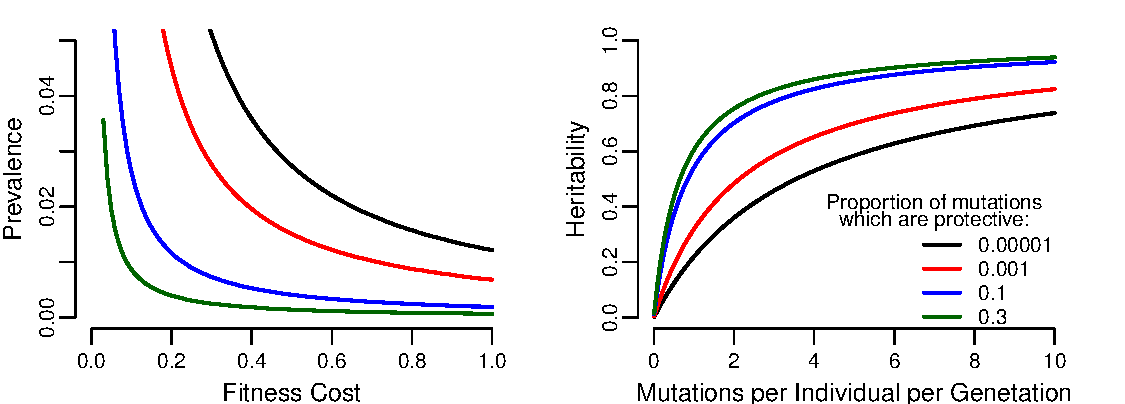
\includegraphics[width=\textwidth]{../figures/SimpleModelSolutions.pdf}
    \caption{Caption goes here}
  \end{figure}
  



\subsubsection*{Specific Aim 1: Relating Population Genetic Processes with the Architecture of Complex Diseases}

I will generalize the basic model from our preliminary results to include the impacts of pleiotropy and environmental and demographic change. In each case, I will solve these generalized models to obtain analytical expressions for the genetic architecture an disease prevalence. In each case, my results will be checked by comparisson to simulations, and in cases where analytical solutions are not tractable, results will be pursued directly via numerical and simulation based methods.


\paragraph{Environmental Change} \qquad

The most straightforward way to incorporate environmental change may also be the most relevant to human disease. The simplest environmental change models are those in which the mean or the variance of the environmental component of the phenotype shifts or increases suddenly. Given the recent and rapid changes to human environments (e.g. diet and lifestyle on type 2 diabetes prevalence), we are most interested in the scenario where an environmental shift has just occurred, but there has not been sufficient time for allele frequencies to evolve away from their previous equilibria. In the case of a shift in the enironmental mean, the effect is simply an increase in prevalence such that $P_{new} = 1 - \Phi\left(\Phi^{-1}\left(1-P_{old}\right)-\delta\right)$, where $\delta$ is the shift in the environmental contribution to liability measured in units of the phenotypic standard deviation ($\Phi$, again, is the Gaussian cdf).

The result of a change in the environmental variance are slightly more complex, as it impacts both the prevalence and the heritability of the disease. The most straightforward impact is on heritability. If the environmental variance is increased by an amount $\psi$, then heritability is decreased such that $h^2_{g,new} = \frac{h^2_{g,old}}{1+\psi}$ (where again, $\psi$ is given here in units of the pre-change phenotypic variance). Prevalence, on the other hand, will increase to $P_{new} = 1 - \Phi\left(\frac{\Phi^{-1}\left(1-P_{old}\right)}{1+\psi}\right)$.
In both of these simple environmental change scenarios, the a given mutation's effect on liability is unchanged. The effect on risk, however, is increased, as a given mutation's contribution to risk conditional on its contribution to liability also depends on the prevalence of the disease (expressions omitted due to space). The result is that the while the additive genetic variance for liability is unchanged under either scenario, we expect that on the \textit{risk} scale it will be increased. A shift in the mean of the environmental contribution should actually cause an increase in heritability on the risk scale, while the impact of an increase in the variance of the environmental contribution on the heritability of risk are not immediately obvious, and may be architecture dependent.

In addition to these simple scenarios, I will also use simulations to study how less recent changes to the environment (e.g. following the Out of Africa event) might have impacted genetic architecture.


% A change in the environmental variance would result in a change in both the prevalence, similar to the mean shift case, as well as they heritability, yielding a means by which the two scenarios may plausibly be distinguished.

\paragraph{Pleiotropy}

As noted in the background above, mounting evidence suggests that genetic variation is often highly pleiotropic. We will consider pleiotropic effects of two kinds. The first includes pleiotropic effects on other disease traits. Pleiotropy of this form will generally act to modulate the additive selection coefficient felt by a given allele. Liability increasing mutations which have protective effects on other diseases will have less strongly negative selection coefficients than in the preliminary model (or may even be selected for), while those which increase liability for multiple diseases will incur additional selective cost beyond that due to direct selection on the focal disease.

The second form of pleiotropy considered will be due to stabilizing selection on continuously distributed (i.e. non-disease) quantitative traits. In models of stabilizing selection on quantitative traits at equilibrium, there is no directional component to the selection felt by individual alleles. Rather, due to variance reducing selection for individuals to cluster near the optimum, individual alleles experience symetric underdominance with respect to fitness (i.e. the minor allele is always selected against), where the strength of selection depends on the effect size of the mutation on the quantitative trait relative to the strength of stabilizing selection \cite{Robertson:1956dk}.

This observation suggests an interesting relationship which will form the foundation for our modeling of pleiotropy. When a mutation effects only disease, selection is directional and additive, whereas when a mutation effects only quantitative traits, selection is underdominant. Mutations which have large effects on disease and smaller impacts on quantitative traits will experience directional selection with the disease causing mutation being partially dominant for fitness, while mutations which have large effects on quantitative traits and smaller effects on disease will be underdominant for fitness, but asymetrically so, with the liability increasing homozygote being less fit than the liability decreasing homozygote.

The major objective here is to derive an expression for joint distribution of effect size and allele frequency (i.e. the genetic architecture) as a function of the parameters ($\Theta_A$) which describe the nature of pleiotropy impacting the disease architecture. These two quantities are conditionally independent of one another given the specification of the selection coefficient(s), which suggests a tractable approach for theoretical analysis and inference (aim 2). The expression for the genetic architecture can be written as an integral over the selection coefficients
\begin{align}
  p\left(\alpha,x \mid \Theta_A\right) = \int \int p\left(\alpha \mid s,h,\Theta_A\right) p\left(x \mid s,h \right) p\left(s,h\right)\mathrm{d}s \mathrm{d}h.
\end{align}
The expression for the distribution of allele frequencies ($p\left(x \mid s,h\right)$) can be computed from standard diffusion theory \cite{Ewens}, and this fact can be leveraged in an inference context (aim 2) to learn the distribution of the selection coeficients ($p\left(s,h\right)$) directly from the data (alternately, plausible distribution can be specified in a theoretical context to understand how differences in the distribution of selection coeffients impact architecture). This leaves specifying the distribution of effect sizes for a given set of selection coefficients and under a given set of parameters governing the effects of pleiotropy ($p\left(\alpha \mid s,h,\Theta_A\right)$) as the primary theoretical task.

I will approach this problem first by considering simple isotropic models of pleiotropy in which mutations may affect more than one disease/trait, but there is no inherent mutational covariance among diseases or traits. In particulary, I will investigate how the number of pleiotropically related diseases/traits, the strength of selection on them, and the degree of functional overlap among diseases/traits all impact the genetic architecture of disease.

% Stated more formally, if we let the relative fitness of the liability decreasing homozygote by equal to 1, then under the standard \{1,1-hs,1-s\} parameterization of fitness
% \begin{align}
%   s &= -2\alpha S\phi\left(\Phi^{-1}\left(1-P\right)\right) + \gamma \left(\Theta_D\right)  \\
%   h &= \frac{1}{2} + \lambda\left(\Theta_Q , \Theta_D\right) \hspace{4cm} \lambda\left(\Theta_Q , \Theta_D\right) > 0
% \end{align}
% where $\Theta_D$ and $\Theta_Q$ represent the parameters describing the nature of the pleiotropic relationship of the focal disease to other diseases $\left(\Theta_D\right)$ and to quantitative traits $\left(\Theta_Q\right)$. These will include features like the number of diseases (or quantitative traits) with pleiotropic effects on the focal disease, their fitenss costs (or the strength of stabilizing selection), and the joint distribution of mutational effects on pleiotropic diseases and traits. The functions $\gamma$ and $\lambda$ represent the distributions of directional selection effects and dominance effects that we expect to arise under a given parameterization of pleiotropy. It is already clear at this juncture that the number of possible choices for exactly how to paraterize pleiotropy is vast, particularly when one takes stock of the possibility for mutational covariances among diseases and traits. We will therefore focus initially on straightforward isotropic cases where e.g. all other diseases have the same parameters as the focal disease and there is no mutational covariance among traits or diseases. I will also benefit from the opportunity to collaborate with a talented graduate student in the Sella lab (Yuval Simmons), who has developed an extensive model of pleiotropy for quantitative traits under stabilizing selection alone, which will allow me to focus predominantly on modeling pleiotropic diseases, and on incorporating the pleiotropic impact of quantitative traits into this model.

% \jb{so this section still hasn't gotten all that close to where it needs to be. The point about stabilizing selection and dominance is a tricky one. I now take your point about expressing things in terms of $p(\alpha \mid s)$, and will take aim at rewriting this section with that in mind next, but I need to pass this along now without waiting any longer. I think ultimately the thing boils down to an expression like the one below (where $\Theta_A$ represents the parameters for both the disease pleiotropy and quantitative trait pleiotropy combined). Unclear if wise to start throwing double integrals at reviewers though?}

% \begin{align}
%   p\left(\alpha_i , x_i \mid \Theta_A \right) = \int_0^1\int_{\frac{1}{2}}^{\frac{1}{s}} p(x_i \mid s_i , h_i ) p\left(h_i \mid s_i , \Theta_Q \right)p\left(\alpha_i \mid s_i , \Theta_A \right)p\left(s_i \mid \Theta_A \right) \mathrm{d}h \mathrm{d} s
%   \end{align}


\paragraph{Non-Equilibrium Demography}


It is clear from population genetic work over the last decade and a half that demographic events such as the Out of Africa bottleneck and recent explosive population growth have had a significant impact on allele frequencies and therefore potentially on genetic architecture. Recent work from Dr Sella's lab\cite{Simons:2014fj}, among others \jb{cite others} suggests that both the bottleneck and recent growth may have impacted genetic architecture, though the relative importance of each depends on the (as yet unknown) selection coefficients of disease alleles. However, what most work to date on this problem has been done in the context of a single site in a vaccum with a fixed selection coefficient, with no explicit disease phenotype, and therefore no model of the relationship between effect size and selection coefficient.

I will use simulation based approaches to study how the particular course of human demographic history has impacted the evolution of complex disease architecture and prevalence. Population size changes impact architecture through their modulation of the relationship between genetic drift and natural selection. All else being equal, genetic architectures in larger populations will be composed of more rare alleles, due to the increased efficiency of selection, though the precise impact depends on the details of the model. My investigation of the preliminary model also suggests that disease prevalence at equilibrium is fairly sensitive to population size. This is significant, specifically because the selection coefficient experienced by a particular allele depends on the disease prevalence. If prevalence evolves over time in response to changes in population size, then selection coefficients will change over time as well.


% A point of particular importance will be understanding the extent to which flucuations in population size are responsible for deviations in the bulk behavior of the population from the equilibrium described in eqn \eqref{univariate-bulk-eq}. While parameters such as the total per individual mutational input ($U^{+/-}$), effect size distributions ($f^{+/-}(\alpha)$, and fitness cost of the disease ($S$) are not sensitive to changes in population size, my investigations of the preliminary model suggest that both the additive genetic variance ($V_A$) and the disease prevalence ($P$) are fairly sensitive to differences in population size at equilibrium (results not shown), which suggests that changes in population size over time may lead to changes in these quantities. This is significant, specifically because the selection coefficient experienced by a particular allele depends on the disease prevalence. If this quantity changes over time, then the selection coefficient experienced by individual alleles will also change over time, and will therefore require a simulation based approach


\subsection*{Specific Aim 2: Inference of Model Parameters from Complex Disease GWAS}

\paragraph{Background}

The existing work which comes closest to that proposed in this aim is recent work applying the Eyre-Walker model (discussed in intro above) to investigate the genetic architecture of complex disease. One such line of work, which includes two studies from David Altshuler's group and colleagues, simulates disease architectures under the Eyre-Walker model, and then compares the number causal type 2 diabetes variants discovered by a given study design to that which would be expected under the Eyre-Walker model simulations, with a particular focus on inferring the total mutational target size and the pleiotropy parameter $\tau$, which captures the coupling between fitness and effect size. These studies used the number of genome wide significant variants \cite{Agarwala:2013bu,Fuchsberger:2016df} as summary statistics in an approximate Bayesian computation (ABC) approach. The initial study\cite{Agarwala:2013bu}, which simply used the total number of variants discovered was able to eliminate the pleiotropic extreme (i.e. the Pritchard model) and a model in which fitness and effect are tightly coupled, but could say little beyond that. A more recent application\cite{Fuchsberger:2016df} used the number of significant variants with minor allele frequency (MAF) < $5\%$, as a summary statistic, and was able to show that relatively small values of $\tau$ in the range of 0.1 (i.e. relatively weak coupling between effect size and fitness) are most consistent with the genetic architecture of type 2 diabetes.

Another study in this vain is that of Mancuso et al (2015)\cite{Mancuso:2015cp}, who used the Eyre-Walker model to investigate the genetic architecture of prostate cancer susceptibility. Rather than using signficant hits as a summary statistic, these authors used variance partitioning methods\cite{Yang:2011hd} to estimate the proportion of the total genetic variance that is attributable to rare alleles ($0.01\% > \text{MAF} > 1\%$), and then took this quantity as the ABC summary statistc. The result was support for moderate values of of $\tau \approx 0.5$.

The results of these studies highlight a couple of important facts. One is the difficulty of interpretting the meaning of the $\tau$ parameter in the Eyre-Walker model. While it is clear that lower values of $\tau$ represent a weaker coupling between fitness and effect size, it remains unclear how to intperpret this parameter biologically, as it was not derived from any explicit model of the impact of pleiotropic traits on the focal trait. The Eyre-Walker model is also fundamental not extensible to inference with multiple traits together, which we expect to particularly important in the future as multi-trait GWAS methods continue to mature.\cite{PickrellPairwise,SomeMatthewStephensPaper}

One encouraging takeaway is the fact that inference approaches which use information about the frequencies of alleles discovered in GWAS\cite{Mancuso:2015cp, Fuchsberger:2016df} obtained more precise parameter estimates than the one that did not\cite{Agarwala:2013bu}, but it is worth stating that all of these studies leave substantial amounts of the information contained in GWAS data unused, indicating that there should be substantial room for improvement. Finally, it should be noted that all of these studies rely on the assumption that the distribution of selection coefficients experienced by disease associated alleles resembles the gamma distribution often assumed for non-synonymous mutations\cite{EyreWalker:2007dl} (though perhaps with little real justification\cite{Racimo:2014cb}), rather than estimating the distribution of selection coefficients from the data directly. It is therefore clear that there is a need for an inference approach which A) uses the totality of the evidence available in GWAS data, and B) allows for the estimation of parameters which have clear biological interpretations, which is the focus of this aim.

% which used population genetic simulations and what is essentially an Approximate Bayesian Computation approach under the Eyre-Walker model described above in order to infer features of the genetic architecture of type 2 diabetes. While these studies have provided valuable insights (in particular, appearing to rule out a role for rare variants in explaining a substantial proportion of heritability), they face some serious limitations. For example, due to their reliance on the Eyre-Walker model for pleiotropy, which has no obvious biological justification, it is difficult to know how to interpret the inference that type 2 diabetes is impacted by an intermediate amount of pleiotropy. They further assume that the distribution of selection coefficients on GWAS variants is similar to that observed for non-synonymous mutations in coding regions, despite the fact that these represent only 10\% of variants associated with type 2 diabetes, and 2-20\% in other GWAS \jb{cite Joe 18 traits functional annotations paper}. Moreoever, the approach uses the number of genome wide significant variants discovered in the GWAS as the lone summary statistic, thereby discarding a great deal of information about architecture that is present in the frequencies of the GWAS variants and the relationship between their frequencies and effect sizes.

% Another class of recent work which bears on these questions is a collection of variance component methods and related approximation to them \jb{cite: LD score regression} which seek to partition heritable variation with respect to minor allele frequency bin \jb{cite Schizophrenia 108 paper; others}. Such methods were developed as a generalization of the variance component methods pioneered in the early part of this decade \jb{cite Yang et al 2011} in order to assess whether 

% applied to demonstrate that variants of a given minor allele frequency range (i.e. 0.4-0.5) make a substantial contribtu

% \jb{Bulik-Sullivan, Finucane, and collaborators}. This framework was originally introduced to measure the impact of non-genetic confounding on the inflation of GWAS summary statistics, but has since been extended to estimate genetic correlations among phenotypes and to partition genetic variance among different functional annotations \jb{cite discrete and condtinuous annotation paper}. This last application seems particularly powerful as a descriptor of the distribution of

\paragraph{Approach}
I will develop an inference approach which leverages GWAS data to infer the parameters of the models developed in Aim 1 for a number of disease GWAS datasets. The approach is based on the Poisson Random Field and related composite likelihood techniques which have been used extensively in population genetic inference. Given 1) the $K$ genome wide significant variants discovered in a GWAS, 2) estimates of their effect sizes and allele frequencies ($\alpha_i$, $x_i$), 3) an estimate of the heritable variation ($V^*_{G,b}$) attributable to each of B minor allele frequency bins, and 4) the parameters of the study $\Theta_S$ (i.e. the number of cases and controls and the disease prevalence assumed for the GWAS), the likelihood of the evolutionary parameters underlying the architecture ($\Theta_A$) can be written as
\begin{multline*}
  L\left(\Theta_A \mid \{\left(\alpha_i, x_i\right)\}_{i=1}^K , \{V^*_{G,b}\}_{b=1}^B, \Theta_S\right) \\
               = Pr\left(K \mid \Theta_A , \Theta_S \right) \left( \prod_{i=1}^K Pr\left(\alpha_i , x_i \mid \Theta_A \right) H\left(\alpha_i , x_i \mid \Theta_S\right) \right) \prod_b Pr\left(V^*_{G,b} \mid \Theta_A, \Theta_S \right)
\end{multline*}
The first term gives the probability of observing $K$ genome wide significant variants associated with the disease (which is Poisson distributed). The second term gives the probability density of a variant with a given effect size and frequency, while the third term gives the power to detect such a variant as a function of the study parameters. The final term gives the probability that a given proportion of the heritability not captured by the $K$ genome wide significant variants is apportioned to a given minor allele frequency bin. The first, second, and fourth terms all depend on the evolutionary parameters ($\Theta_A$) and therefore are the major link which connects Aim 1 and Aim 2, as the the theory from Aim 1 will be used to compute these expressions.

Intuitively, the number of genome wide significant variants mostly provides information about the mutational target size, while their frequencies are informative about the strength of selection they experience, and the relationship between frequency and effect size is therefore informative about the nature of the pleiotropic effects of disease associated loci.

The proportion of the ``missing heritability'' attributable to different minor allele frequency bins essentially contains information about the mean strength of selection experienced by disease variants, and therefore helps constrain the range of possible models which can fit the data. It is a less rich source of information than the individual genome-wide significant variants themselves, as we do not get to observe informative features such as whether it is the derived or ancestral allele which increases disease risk, and we must fold the frequency spectrum, which in particular discards information about protective mutations\cite{Bustamante:2001wi}. Nevertheless, the theory from Aim 1 will make predictions about how variance is distributed across minor allele frequencies \jb{hopefully add a figure here to show how two different choices of evolutionary parameters lead to different distributions of variance among bins}, which means it can be used for inference. Intuitively, the stronger seletion on disease variants is, the larger the proportion of variance we expect to be explained by low frequency bins.


The likelihood above is a composite rather than a true likelihood, meaning that it does not account for the non-indepdendence (i.e. linkage disequilibrium) among sites. Such approaches are commonplace in population genetics when full likelihood computation is infeasible. Composite likelihoods have the property that they are unbiased with respect to the maximum likelihood estimate, but understate the uncertainty about that estimate, precisely because non-independence among datapoints is ignored, leading to the appearance of stronger evidence than actually exists, and naive approaches to model comparison therefore erroneously tend to favor more complex models \jb{Gao and Song 2010}. This limitation can be overcome by bootstrapping or potentially by adapting recently developed methods from the literature on demographic inference which show promise in circumventing these issues analytically at significantly reduced computational cost. 


% message from Kristin about composite likelihood stuff
% This composite likelihood ignores the correlation in allele frequencies (linkage disequilibrium) between neutral sites. Thus it is an approximation to the true likelihood. As it ignores dependence between obser- vations, the composite likelihood surface will be too peaked. A number of authors have taken composite- likelihood approach to inferring a range of population genetic parameters (e.g. Hudson (2001); see Larribe and Fearnhead (2011); Varin et al. (2011) for a broader statistical views on composite likelihood). In the setting of inferring genome-wide parameters, e.g. parameters of neutral demographic models, the maximum composite likelihood parameter estimates are known to be consistent in the limit of many unlinked genomic regions (Wiuf, 2006). Composite likelihood approaches have also been used in the context of selective sweeps, starting with (Kim and Stephan, 2002) who take a composite likelihood formed like eqn (17) of the product of marginal probabilities of allele frequencies within a single population moving away from a proposed selected site (an approach expanded on by Kim and Nielsen, 2004; Nielsen et al., 2005; Chen et al., 2010; DeGiorgio et al., 2014; Racimo, 2016). While in general composite-likelihood methods perform well, in all of these settings typical measures of uncertainty of parameters (confidence intervals) and model choice methods (e.g. AIC) are undermined by the over peakiness of the likelihood.
% With helpful refs
% I think this is other paper: https://academic.oup.com/mbe/article/33/2/591/2579696/Computationally-Efficient-Composite-Likelihood

% \subsection*{Specific Aim 3: Extension to Multi-Ethnic GWAS}

% \paragraph{Background}
% One of the major hoped for uses of disease GWAS data is in the construction of so-called ``polygenic predictors'', which integrate information across a large number of loci (both genome wide significant and not) in order to  forecast an individual's probability of developing a given complex disease. At present, the prediction accuracy of such methods is generally low (though it now exceeds family history as a predictor for some diseases in some situations \jb{cite: definitely schizophrenia I think}), but is expected to increase as sample sizes increase and statistical methods for prediction improve.

% A major limitation already being encountered, however, is that the utility of a given genetic preditor seems to depend somewhat strongly on how closely related the individuals who's risk is being predicted are to the those used to construct the predictor\cite{Martin:2016be}. There are many good reasons for why this might be. Changes in the structure of linkage disequilibrium across populations may lead to ineffective tagging of causal variants in diverged populations, differences in the environment may cause actual differences in the effects of causal variants (i.e. gene-by-environment interaction), or adaptation in one ore more quantitative traits that are genetically correlated with disease may have significantly altered the genetic risk profile across populations.

% The totality of the among population genetic prediction problem (and indeed each possible explanation given above) is beyond the scope of this proposal, but any complete accounting will first require that we understand how we would expect genetic predictors to behave when applied across populations in the absense of any of the above confounding effects. In this case, we still would expect prediction accuracy to decay with evolutionary divergence, simply due to the divergence of genetic architectures among populations under the influence of natural selection and genetic drift. The rate of this divergence, however, will depend on the selection coefficients experienced by disease associated alleles. The theoretical models developed in Aim 1 and inferences derived from Aim 2 will therefore provide the necessary building blocks with which to approach the problem, and I will apply the results of these aims to make predictions about the theoretical maximum accurary that can be obtained for a genetic predictor constructed in one population when applied to an evolutionarily diverged one. 

% \paragraph{Approach}

% The theoretical maximum prediction accuracy possible when applying a predictor trained in one population ($X$) to some evolutionarily diverged population ($Y$), depends on the amount of genetic variance in population $Y$ that can be explained by alleles which are polymorphic in population $X$ (and therefore plausibly detectable in GWAS), the amount of genetic variance that is private to population $Y$, and the environmental contribution to variance in population $Y$. If we denote these three quantities $V_A^{Y\mid X}$, $V_A^{Y_P}$, and $V_E^Y$ respectively, then the maximum achievable prediction accuracy of a predictor trained in $X$ and applied in $Y$ is $\frac{V_A^{Y \mid X}}{V_A^{X \mid Y} + V_A^{Y_P} + V_E^Y}$.

% In general, the contribution that alleles in a given set $W$ make to genetic variance can be expressed as

% \begin{align}
%   V_A^{W} = \int_0^1 \int_{-\infty}^{\infty} \alpha^2 x \left(1-x\right) p_{W}\left(\alpha,x\right) \mathrm{d}\alpha \mathrm{d}x
%  \end{align}
%  where $p_{W}\left(\alpha,x\right)$ is the joint distribution on frequency and effect size for allele in that set. In our case, we have two different sets of alleles, and so we will need this joint distribution in $Y$ conditional on segregation in $X$ ($p_{Y\mid X}\left(\alpha, x_Y \right)$), and conditional on absence in $X$ ($p_{Y_P}\left(\alpha,x_{Y}\right)$). Each of these can be obtained by combining the results of our modeling and inference efforts in Aims 1 and 2 with simulation of allele frequency trajectories from conditional diffusion processes. For example, given that an allele is observed at frequency $x_X$ in population $X$ with effect size $\alpha$, we can determine the distribution of possible frequencies it might take in population $Y$ ($p\left(x_Y \mid s , x_X\right)$) by simulating the diffusion process backward in time to the point where the two populations split, and then forward in time to population $Y$ in the present day \jb{probably a small figure to illustrate this}. We can combine this with the distribution of selection coefficients inferred in Aim 2 ($p\left(s\right)$), and our model from Aim 1 for the relationship between effect size and selection coefficient ($p\left(\alpha \mid s \right)$) \jb{I need to actually write that part} to obtain an expression for the joint distribution of frequency and effect size in population $Y$ conditional on segregation in population $X$

%  \begin{align}
%    p_{Y \mid X}\left(\alpha , x_Y \right) = \int_0^1 p\left(\alpha \mid s \right) p\left(x_Y \mid s, x_X\right)p\left(s\right)\mathrm{d}s.
% \end{align}
% The process for obtaining $p_{Y_P}\left(\alpha, x_Y\right)$ is similar, but slightly more involved, because we must also account for new mutations segregating in $Y$ which have occured since the split with $X$, as well as sites where the derived mutation has fixed in $X$ but is still polymorphic in $Y$.

% One obvious potential pitfall in this approach is that our inferences from GWAS may only provide incomplete information about the distribution of selection coefficients, as the most significant GWAS variants are likely to experience similar selection coefficients. However, we will still be able to make statements about the absolute decrease in prediction accuracy attributable to variants with selection coefficients in this range, and by making plausible assumptions about the range and distribution of selection coefficients of additional 

% \jb{so this obviously frays at the end and needs to be wrapped up, but think it's more worthwhile to send along as is now. It clearly still needs work, but think I can make this work (at least for the proposal). It's probably far too zoomed in, but I can try to pull it back out to a higher level on my next rewrite}
  
% Ultimately, this is a question of how much of the variance in disease risk in one population can be explained by loci which contribute to variance in another. Answering this question requires an understanding of the behavior of allele frequency trajectories 

% For example, due to linkage disequilibrium which is pervasive at short physical scales in human populations, each genome wide significant variant in a GWAS actually represnts a small cluster of variants which all have elevated association statistics, presumably one of which is the actualy true causal variant. 

% To date, the vast majority of genome wide association studies have been performed in populations of European ancestry, and it remains an open question in medical genetics to what extent GWAS results from one population or region will be applicable or useful in another evolutionarily diverged population. While this disparity is unlikely to be entirely resolved any time soon due to vast structural issues in the field, there has been a growing call for a diversification of GWAS to broader ancestry cohorts



% This aim proposed to quantitatively address two major questions related to the application of GWAS results across populations: 1) how do the theoretical upper limits of genetic prediction accuracy depend on the underlying evolutionary parameters which govern genetic architecture and 2) to what extent will access to GWAS of multiple cohorts of divergent ancestry improve our ability to make inferences about the genetic architecture of complex disease.



\bibliography{library}
\bibliographystyle{unsrt}
\end{document}
